
\section{局部闭嵌入与局部闭子概形}

既然已经定义了开子集与闭子集的类似物，自然而然就该定义局部闭子集的类似物了。回想：局部闭子集是开子集与闭子集的交。因此它们是开子集的闭子集，或者等价地，是闭子集的开子集。这些等价性在概形的国度里将会有一点麻烦。（类似地，子群与商群这两个观念也不太互补。设问：群 $G$ 的「\trSubquotient」应当定义为 $G$ 的商的\trSubgroup，还是 $G$ 的\trSubgroup{}的\trQuotient？抑或二者是同一回事？在定义\trLocally\trClosedEmbedding{}时，我们将会正面撞上同一个问题。）

我们称一个\trMorphism{} $\pi\colon X\to Y$ 是\textbf{\trLocally\trClosedEmbedding}（locally closed embedding；或\textbf{\trLocally\trClosedImmersion}，locally closed immersion），若 $\pi$ 可以分解为
\[
X\xhookrightarrow[\text{\trClosed}]{\ \rho\ } Z\xhookrightarrow[\text{\trOpen}]{\ \tau\ } Y,
\]
其中（正如所标注的那样）$\rho$ 是一个\trClosedEmbedding，而 $\tau$ 是一个\trOpenEmbedding。例如，由 $(x,y)\mapsto(t,0)$ 给出的\trMorphism{} $\Spec k[t,t^{-1}]\to\Spec k[x,y]$ 就是一个\trLocally\trClosedEmbedding（图~\ref{fig:locally-closed-embedding}）。符号 $\hookrightarrow$ 常被用来表示一个态射是\trLocally\trClosedEmbedding。由于\trClosedEmbedding{}与\trOpenEmbedding{}都是\trMonomorphism（分别是练习~9.1.J 与\cref{ex:open-embeddings-are-monomorphisms}），而\trMonomorphism{}对\trComposition{}保持，所以\trLocally\trClosedEmbedding{}也是\trMonomorphism。

\begin{figure}[htbp]
\centering
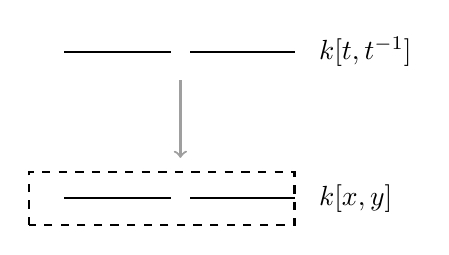
\begin{tikzpicture}[scale=0.9,line width=0.8pt]
  \draw (0,2.55) -- (1.50,2.55);
  \draw (1.78,2.55) -- (3.25,2.55);
  \node[anchor=west] at (3.45,2.55) {$\Spec k[t,t^{-1}]$};
  \draw[gray!75,->] (1.64,2.15) -- (1.64,1.05);
  \draw[dashed] (-0.50,0.10) rectangle (3.25,0.85);
  \draw (0,0.48) -- (1.50,0.48);
  \draw (1.78,0.48) -- (3.25,0.48);
  \node[anchor=west] at (3.45,0.48) {$\Spec k[x,y]$};
\end{tikzpicture}
\caption{局部闭嵌入 $\Spec k[t,t^{-1}]\to\Spec k[x,y]$（$t\mapsto(t,0)=(x,y)$，亦即 $(x,y)\mapsto(t,0)$）。（依原书手绘图重绘。）}\label{fig:locally-closed-embedding}
\end{figure}

（警告：术语\emph{浸入}常被用来指\emph{\trLocally\trClosedEmbedding}或\emph{\trLocally\trClosedImmersion}，但这是不明智的术语——理由在定义~9.1.1 处谈\trClosedEmbedding{}时就已出现：微分几何中的浸入观念，更接近代数几何学家所称的\trUnramified，我们将在 \S21.7 中给出它的定义。此外，光杆的术语\emph{嵌入}也应当避免，因为它不必要地不精确。）

\textbf{9.2.1.}\quad 若 $X$ 是 $Y$ 的一个子集（且 $\pi$ 在集合的层面上就是包含映射），我们就说 $X$ 是 $Y$ 的一个\textbf{\trLocally\trClosedSubscheme}。（警告：光杆的术语\textbf{\trSubscheme}常被用来意指\emph{\trLocally\trClosedSubscheme}，但我们将避免这种令人不快的用法。）

\textbf{9.2.A.（容易的练习）}\quad 证明：\trLocally\trClosedEmbedding{}都\trLocally\trFiniteType。

\textbf{9.2.B.（练习）}\quad 设 $\pi\colon X\to Y$ 是一个\trLocally\trClosedEmbedding，其像为 $Y$ 的一个\trClosedSubset。证明：$\pi$ 是一个\trClosedEmbedding。一条可能的提示：「是\trClosedEmbedding」这一性质是对目标仿射局部的，练习~9.1.D。（这在哲理上是很有用的；例如见 \S11.2.2。）

写到这里，你其实可以顺手定义概形 $X$ 中两个\trLocally\trClosedEmbedding{}的交（它也将是 $X$ 中的一个\trLocally\trClosedEmbedding）。但这会相当别扭，因为你将不得不证明：你的构造不依赖于每个\trLocally\trClosedEmbedding{}之分解为一个\trClosedEmbedding{}与一个\trOpenEmbedding{}时的具体方式。我们不如按兵不动，且等到\mbox{练习~10.2.C}——届时，把交认作一个\trFiberProduct{}将会使这件事容易得多。

显然，$X$ 的一个\trClosedSubscheme{} $V$ 的\trOpenSubscheme{} $U$ 可以解读为某个\trOpenSubscheme{}的\trClosedSubscheme：由于 $V$ 上的拓扑是从 $X$ 的拓扑诱导而来的，$U$ 的底集合是 $X$ 的某个\trOpenSubset{} $U'$ 与 $V$ 的交。我们可以取 $V'=V\cap U'$，于是 $V'\hookrightarrow U'$ 是一个\trClosedEmbedding，而 $U'\hookrightarrow X$ 是一个\trOpenEmbedding。

而一个\trOpenSubscheme{} $U'$ 的\trClosedSubscheme{} $V'$ 能否表达为某个\trClosedSubscheme{} $V$ 的\trOpenSubscheme，却并不清楚。在拓扑空间的\trCategory{}中，我们会取 $V$ 为 $V'$ 的\trClosure；因此，如今我们便有动机去定义一个类似的构造——这也给了我们一个名正言顺的借口，好在 \S9.4 中引入几个相关的观念。随后，我们将在好的情形（例如 $X$ \trNoetherian{}时）于\mbox{练习~9.4.C}中解决这个问题。

我们把这段讨论在一道练习中正式化。

\textbf{9.2.C.（练习）}\quad 设 $V\to X$ 是一个\trMorphism。考虑三个条件：
\begin{enumerate}[label=(\roman*)]
\item $V$ 是 $X$ 的一个\trOpenSubscheme{}与一个\trClosedSubscheme{}的交（你得自行定义这里「交」的含义；见\cref{ex:open-embeddings-base-change}，或者看下面的提示）。
\item $V$ 是 $X$ 的某个\trClosedSubscheme{}的\trOpenSubscheme，也就是说，$V$ 分解为一个\trOpenEmbedding{}接一个\trClosedEmbedding。
\item $V$ 是 $X$ 的某个\trOpenSubscheme{}的\trClosedSubscheme，也就是说，$V$ 是一个\trLocally\trClosedEmbedding。
\end{enumerate}
证明：(i) 与 (ii) 等价，且二者都蕴含 (iii)。（注记：(iii) 并\emph{不}总是蕴含 (i) 与 (ii)；病态的例子见 [Stacks, tag 01QW]。）提示：按下面这样来想问题或许有帮助。你可能希望把一个\trLocally\trClosedEmbedding{}想成一个\trCartesianDiagram。
\[
\begin{tikzcd}[row sep=3.2em, column sep=6.5em]
V \ar[r, hook, "\text{\trOpenEmbedding}"] \ar[d, hook, "\text{\trClosedEmbedding}"] & K \ar[d, hook, "\text{\trClosedEmbedding}"'] \\
U \ar[r, hook, "\text{\trOpenEmbedding}"'] & X
\end{tikzcd}
\]
（我们已经知道：与\trOpenEmbedding{}作\trFiberProduct{}是存在的，见\cref{ex:open-embeddings-base-change}。）把 (i) 解读为这条图示的存在性；把 (ii) 解读为这条图示去掉左下角；把 (iii) 解读为这条图示去掉右上角。

\textbf{9.2.D.（练习）}\quad 证明：两个\trLocally\trClosedEmbedding{}的\trComposition{}仍是\trLocally\trClosedEmbedding。（提示：你或许可以用上一道练习中的「(ii) 蕴含 (iii)」。）

\textbf{9.2.2.}\ \emph{不重要但好玩的注记。}\quad 在\trLocally\trClosedEmbedding{}的定义中，我们不得不做出一个选择（取「一个\trClosedEmbedding{}接一个\trOpenEmbedding」的分解，而不是反过来），这也许让人觉得别扭；但这一类问题早先就出现过：一个群的\trSubquotient{}既可以定义为\trSubgroup{}的\trQuotient，也可以定义为\trQuotient{}的\trSubgroup。哪个才是正确的定义？抑或二者是同一回事？（提示：子商的子商当然应当还是子商，参看练习~9.2.D。）
